% -----------------------------------------------------------------------
\section{Marco Teórico}
\label{sec:marco}

Esta sección presenta, en su forma estándar, las formulaciones de los cinco
problemas abordados y los tres niveles de Búsqueda Tabú implementados.

\subsection{Formulaciones matemáticas}

\subsubsection{Mochila 0/1 (Knapsack)}
Dados $n$ ítems con pesos $w_i > 0$, ganancias $p_i > 0$ y capacidad
$W$, se definen variables binarias $x_i \in \{0,1\}$.
La formulación empleada sigue el modelo clásico de Martello y
Toth~\cite{martello1990knapsack}, utilizado también por
Pisinger~\cite{pisinger2005hard} en los benchmarks de este trabajo:

\begin{align}
  \max        \quad & \sum_{i=1}^{n} p_i\, x_i \label{eq:kp_obj}\\
  \text{s.a.} \quad & \sum_{i=1}^{n} w_i\, x_i \leq W \label{eq:kp_cap}\\
                    & x_i \in \{0,1\}, \quad i = 1,\ldots,n \notag
\end{align}

La restricción~\eqref{eq:kp_cap} garantiza que el peso total no supere
la capacidad.
El problema es $\mathcal{NP}$-duro en general~\cite{garey1979computers},
aunque admite solución exacta en tiempo pseudopolinomial mediante
programación dinámica.

\subsubsection{TSP}
El Problema del Viajante consiste en encontrar el ciclo hamiltoniano de
costo mínimo en un grafo completo ponderado.
La formulación empleada sigue el modelo de Dantzig, Fulkerson y
Johnson~\cite{dantzig1954solution}.
Sea $G=(V,E,d)$ un grafo completo con $|V|=n$ nodos y distancias
$d_{ij}$.
Se definen $x_{ij} \in \{0,1\}$ (el arco $(i,j)$ pertenece al tour):

\begin{align}
  \min        \quad & \sum_{i \neq j} d_{ij}\, x_{ij} \label{eq:tsp_obj}\\
  \text{s.a.} \quad & \sum_{j \neq i} x_{ij} = 1,
                      \quad \forall i \in V \label{eq:tsp_out}\\
                    & \sum_{i \neq j} x_{ij} = 1,
                      \quad \forall j \in V \label{eq:tsp_in}\\
                    & \sum_{i \in S,\, j \notin S} x_{ij} \geq 1,
                      \quad \forall S \subsetneq V,\; 2 \leq |S| \leq n-2
                      \label{eq:tsp_sub}\\
                    & x_{ij} \in \{0,1\} \notag
\end{align}

Las restricciones~\eqref{eq:tsp_out}--\eqref{eq:tsp_in} garantizan que
cada nodo tenga exactamente un arco entrante y uno saliente.
La restricción~\eqref{eq:tsp_sub} (subtour elimination de Dantzig,
Fulkerson y Johnson) asegura un único ciclo hamiltoniano~\cite{applegate2006traveling}.

\subsubsection{CVRP}
El Problema de Ruteo de Vehículos con Capacidad extiende el TSP a múltiples
rutas, cada una operada por un vehículo de capacidad limitada~$Q$.
La formulación empleada sigue el modelo de Laporte~\cite{laporte1992vehicle};
el uso de Búsqueda Tabú para el CVRP fue sistematizado en~\cite{cordeau2002guide}.
Para una referencia integral sobre VRP véase~\cite{toth2002vehicle}.
Sea $V = \{0,1,\ldots,n\}$ donde el nodo $0$ es el depósito.
Se dispone de $K$ vehículos idénticos de capacidad $Q$.
Variables: $x_{ij} \in \mathbb{Z}_{\geq 0}$ (número de veces que
algún vehículo recorre $(i,j)$).
La Figura~\ref{fig:tsp_cvrp} contrasta la estructura de una solución de
ambos problemas de ruteo.

\begin{figure}[t]
  \centering
  \begin{tikzpicture}[x=0.95cm, y=0.95cm,
      nodo/.style={circle, draw, fill=gray!20, inner sep=0pt,
                   minimum size=5pt},
      dep/.style={rectangle, draw, fill=black, inner sep=0pt,
                  minimum size=6.5pt},
      ruta/.style={thick, ->, >=stealth}]
    % (a) TSP: un único ciclo hamiltoniano
    \begin{scope}
      \foreach \i/\x/\y in {1/0.2/0.3, 2/1.3/0.0, 3/2.4/0.5, 4/2.7/1.7,
                            5/1.7/2.5, 6/0.5/2.3, 7/-0.1/1.3}
        \node[nodo] (t\i) at (\x,\y) {};
      \foreach \a/\b in {1/2, 2/3, 3/4, 4/5, 5/6, 6/7, 7/1}
        \draw[ruta] (t\a) -- (t\b);
      \node[font=\scriptsize] at (1.3,-0.65) {(a) TSP: un tour};
    \end{scope}
    % (b) CVRP: K rutas que parten y terminan en el depósito
    \begin{scope}[xshift=4.3cm]
      \node[dep] (d) at (1.3,1.25) {};
      \node[font=\tiny, below right=-1pt of d] {0};
      \foreach \i/\x/\y in {1/0.0/2.3, 2/0.9/2.7, 3/1.9/2.5,
                            4/2.8/1.7, 5/2.9/0.6, 6/2.0/0.0,
                            7/0.6/0.0, 8/-0.2/0.6, 9/-0.3/1.4}
        \node[nodo] (c\i) at (\x,\y) {};
      \draw[ruta] (d) -- (c1);  \draw[ruta] (c1) -- (c2);
      \draw[ruta] (c2) -- (c3); \draw[ruta] (c3) -- (d);
      \draw[ruta, dashed] (d) -- (c4);  \draw[ruta, dashed] (c4) -- (c5);
      \draw[ruta, dashed] (c5) -- (c6); \draw[ruta, dashed] (c6) -- (d);
      \draw[ruta, densely dotted] (d) -- (c7);
      \draw[ruta, densely dotted] (c7) -- (c8);
      \draw[ruta, densely dotted] (c8) -- (c9);
      \draw[ruta, densely dotted] (c9) -- (d);
      \node[font=\scriptsize] at (1.3,-0.65) {(b) CVRP: $K=3$ rutas};
    \end{scope}
  \end{tikzpicture}
  \caption{Estructura de una solución de ruteo. (a)~En el TSP, un único
           tour visita todos los nodos. (b)~En el CVRP, los clientes se
           reparten en $K$ rutas que parten y terminan en el depósito
           (cuadrado negro), sin exceder la capacidad $Q$ de cada vehículo.}
  \label{fig:tsp_cvrp}
\end{figure}

\begin{align}
  \min        \quad & \sum_{i=0}^{n}\sum_{j=0}^{n} d_{ij}\, x_{ij}
                      \label{eq:vrp_obj}\\
  \text{s.a.} \quad & \sum_{j=1}^{n} x_{0j} = K
                      \label{eq:vrp_k}\\
                    & \sum_{i=0}^{n} x_{ij} = \sum_{k=0}^{n} x_{jk} = 1,
                      \quad \forall j \in V \setminus \{0\}
                      \label{eq:vrp_flow}\\
                    & \sum_{i \in S,\, j \in S} x_{ij}
                      \leq |S| - \left\lceil \frac{\sum_{i \in S} q_i}{Q}
                      \right\rceil,\;
                      \forall S \subseteq V\!\setminus\!\{0\}
                      \label{eq:vrp_cap}\\
                    & x_{ij} \geq 0 \notag
\end{align}

La restricción~\eqref{eq:vrp_k} controla el número de rutas.
La restricción~\eqref{eq:vrp_flow} garantiza conservación de flujo en
cada cliente.
La restricción~\eqref{eq:vrp_cap} elimina sub-tours y aplica la
capacidad vehicular~\cite{dantzig1959truck}.

\subsubsection{Permutation Flowshop Scheduling}
En el Flowshop Permutacional, $n$ trabajos deben procesarse en $m$ máquinas
dispuestas en serie; todos los trabajos siguen la misma secuencia de máquinas
y cada máquina atiende un trabajo a la vez.
El objetivo es minimizar el \emph{makespan}~$C_{n,m}$, es decir, el tiempo
de finalización del último trabajo en la última máquina~\cite{pinedo2016scheduling}.
La formulación recursiva empleada sigue el modelo estándar descrito por
Pinedo~\cite{pinedo2016scheduling} y utilizado por
Taillard~\cite{taillard1993benchmarks} en sus benchmarks.
Sean $n$ trabajos y $m$ máquinas.
Dada una permutación $\sigma$ de los trabajos, se denota
$p_{\sigma(i),j}$ el tiempo de proceso del $i$-ésimo trabajo en la
máquina $j$, y $C_{ij}$ su tiempo de terminación:

\begin{align}
  \min \quad & C_{n,m} \label{eq:fsp_obj}\\
  \text{s.a.}\quad
             & C_{1,1} = p_{\sigma(1),1} \notag\\
             & C_{i,1} = C_{i-1,1} + p_{\sigma(i),1},
               \quad i = 2,\ldots,n \label{eq:fsp_m1}\\
             & C_{1,j} = C_{1,j-1} + p_{\sigma(1),j},
               \quad j = 2,\ldots,m \label{eq:fsp_j1}\\
             & C_{i,j} \geq \max(C_{i-1,j},\, C_{i,j-1})
               + p_{\sigma(i),j},\quad i{\geq}2,\,j{\geq}2
               \label{eq:fsp_dp}
\end{align}

La relación~\eqref{eq:fsp_dp} captura la dependencia doble: un trabajo
no puede iniciar en la máquina $j$ hasta que termine en $j{-}1$ y la
máquina $j$ quede libre del trabajo anterior~\cite{taillard1993benchmarks}.
La Figura~\ref{fig:flowshop_gantt} ilustra esta dependencia para una
permutación de tres trabajos.

\begin{figure}[t]
  \centering
  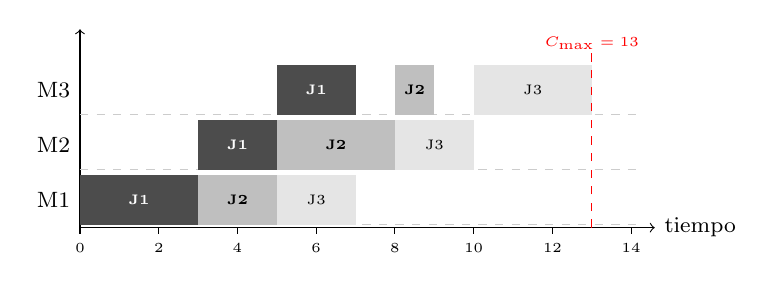
\begin{tikzpicture}[x=0.5cm, y=0.7cm]
    % Ejes
    \draw[->] (0,0) -- (14.6,0) node[right]{\footnotesize tiempo};
    \draw[->] (0,0) -- (0,3.6);
    % Etiquetas máquinas
    \foreach \m/\y in {M1/0.5, M2/1.5, M3/2.5}{
      \node[left, font=\footnotesize] at (0,\y) {\m};
      \draw[dashed, gray!40] (0,\y-0.45) -- (14.2,\y-0.45);
    }
    % J1 (negro): M1[0-3], M2[3-5], M3[5-7]
    \fill[black!70] (0,0.05) rectangle (3,0.95);
    \fill[black!70] (3,1.05) rectangle (5,1.95);
    \fill[black!70] (5,2.05) rectangle (7,2.95);
    % J2 (gris medio): M1[3-5], M2[5-8], M3[8-9]
    \fill[gray!50] (3,0.05) rectangle (5,0.95);
    \fill[gray!50] (5,1.05) rectangle (8,1.95);
    \fill[gray!50] (8,2.05) rectangle (9,2.95);
    % J3 (gris claro): M1[5-7], M2[8-10], M3[10-13]
    \fill[gray!20] (5,0.05) rectangle (7,0.95);
    \fill[gray!20] (8,1.05) rectangle (10,1.95);
    \fill[gray!20] (10,2.05) rectangle (13,2.95);
    % Etiquetas trabajos
    \node[white, font=\tiny\bfseries] at (1.5,0.5) {J1};
    \node[white, font=\tiny\bfseries] at (4,1.5)   {J1};
    \node[white, font=\tiny\bfseries] at (6,2.5)   {J1};
    \node[font=\tiny\bfseries] at (4,0.5)   {J2};
    \node[font=\tiny\bfseries] at (6.5,1.5) {J2};
    \node[font=\tiny\bfseries] at (8.5,2.5) {J2};
    \node[font=\tiny] at (6,0.5)    {J3};
    \node[font=\tiny] at (9,1.5)    {J3};
    \node[font=\tiny] at (11.5,2.5) {J3};
    % Ticks tiempo
    \foreach \t in {0,2,...,14}
      \draw (\t,0) -- (\t,-0.12) node[below,font=\tiny]{\t};
    % Makespan
    \draw[red, dashed] (13,0) -- (13,3.2);
    \node[red, font=\tiny] at (13,3.35) {$C_{\max}=13$};
  \end{tikzpicture}
  \caption{Ejemplo de diagrama de Gantt para Flowshop Permutacional con
           3 trabajos y 3 máquinas, para la permutación
           $\sigma=(\text{J1},\text{J2},\text{J3})$. Todos los trabajos
           recorren las máquinas en el mismo orden (M1, M2, M3) y cada
           máquina los procesa en el orden de $\sigma$; el makespan es
           $C_{\max}=13$.}
  \label{fig:flowshop_gantt}
\end{figure}

\subsubsection{Job Shop Scheduling}
\label{sssec:jobshop}

\begin{figure}[H]
  \centering
  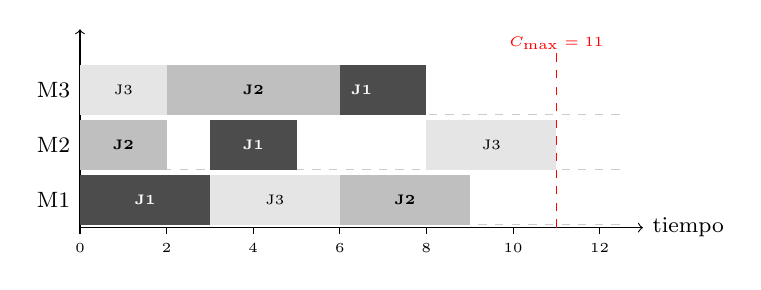
\begin{tikzpicture}[x=0.55cm, y=0.7cm]
    % Ejes
    \draw[->] (0,0) -- (13,0) node[right]{\footnotesize tiempo};
    \draw[->] (0,0) -- (0,3.6);
    % Etiquetas máquinas
    \foreach \m/\y in {M1/0.5, M2/1.5, M3/2.5}{
      \node[left, font=\footnotesize] at (0,\y) {\m};
      \draw[dashed, gray!40] (0,\y-0.45) -- (12.5,\y-0.45);
    }
    % J1 (negro): M1[0-3], M2[3-5], M3[5-8]
    \fill[black!70] (0,0.05) rectangle (3,0.95);
    \fill[black!70] (3,1.05) rectangle (5,1.95);
    \fill[black!70] (5,2.05) rectangle (8,2.95);
    % J2 (gris medio): M2[0-2], M3[2-6], M1[6-9]
    \fill[gray!50] (0,1.05) rectangle (2,1.95);
    \fill[gray!50] (2,2.05) rectangle (6,2.95);
    \fill[gray!50] (6,0.05) rectangle (9,0.95);
    % J3 (gris claro): M3[0-2], M1[3-6], M2[5-8]
    \fill[gray!20] (0,2.05) rectangle (2,2.95);
    \fill[gray!20] (3,0.05) rectangle (6,0.95);
    \fill[gray!20] (8,1.05) rectangle (11,1.95);
    % Etiquetas trabajos
    \node[white, font=\tiny\bfseries] at (1.5,0.5) {J1};
    \node[white, font=\tiny\bfseries] at (4,1.5)   {J1};
    \node[white, font=\tiny\bfseries] at (6.5,2.5) {J1};
    \node[font=\tiny\bfseries] at (1,1.5)  {J2};
    \node[font=\tiny\bfseries] at (4,2.5)  {J2};
    \node[font=\tiny\bfseries] at (7.5,0.5){J2};
    \node[font=\tiny] at (1,2.5)   {J3};
    \node[font=\tiny] at (4.5,0.5) {J3};
    \node[font=\tiny] at (9.5,1.5) {J3};
    % Ticks tiempo
    \foreach \t in {0,2,...,12}
      \draw (\t,0) -- (\t,-0.12) node[below,font=\tiny]{\t};
    % Makespan
    \draw[red, dashed] (11,0) -- (11,3.2);
    \node[red, font=\tiny] at (11,3.35) {$C_{\max}=11$};
  \end{tikzpicture}
  \caption{Ejemplo de diagrama de Gantt para Job Shop con 3 trabajos (J1, J2, J3)
           y 3 máquinas (M1, M2, M3).
           Cada trabajo sigue su propia secuencia de máquinas; el makespan
           $C_{\max}=11$ es el objetivo a minimizar.}
  \label{fig:jobshop_gantt}
\end{figure}

El Job Shop generaliza el Flowshop al permitir que cada trabajo tenga
su propia secuencia de máquinas.
A diferencia del Flowshop, no existe un orden global de máquinas: cada
trabajo $i$ define una ruta particular, y cada máquina puede procesar
a lo sumo un trabajo a la vez.
Cada trabajo $i \in \{1,\ldots,n\}$ tiene una secuencia propia de
operaciones $O_{i1},\ldots,O_{im_i}$ en máquinas $\mu_{i1},\ldots,\mu_{im_i}$.
Sea $s_{ik}$ el tiempo de inicio de la operación $k$ del trabajo $i$ y
$p_{ik}$ su duración.
Se introducen variables binarias $y_{ijk} \in \{0,1\}$ que indican si
el trabajo $i$ precede al trabajo $j$ en la máquina $k$:

\begin{align}
  \min \quad & C_{\max} \label{eq:jsp_obj}\\
  \text{s.a.}\quad
             & C_{\max} \geq s_{i,m_i} + p_{i,m_i},
               \quad \forall i \label{eq:jsp_cmax}\\
             & s_{i,k+1} \geq s_{ik} + p_{ik},
               \quad \forall i,\,k < m_i \label{eq:jsp_prec}\\
             & s_{jk} \geq s_{ik} + p_{ik} - M(1-y_{ijk}),
               \quad \forall i{\neq}j,\,\forall k \label{eq:jsp_dis1}\\
             & s_{ik} \geq s_{jk} + p_{jk} - M\,y_{ijk},
               \quad \forall i{\neq}j,\,\forall k \label{eq:jsp_dis2}\\
             & s_{ik} \geq 0,\quad y_{ijk} \in \{0,1\} \notag
\end{align}

Las restricciones~\eqref{eq:jsp_prec} imponen la precedencia dentro de
cada trabajo.
Las restricciones~\eqref{eq:jsp_dis1}--\eqref{eq:jsp_dis2} son las
disyunciones de máquina: en cada máquina solo un trabajo puede procesar
a la vez ($M$ es una constante suficientemente
grande)~\cite{manne1960job,garey1976complexity}.
La Figura~\ref{fig:jobshop_gantt} ilustra un ejemplo de planificación
con tres trabajos y tres máquinas.


\begin{table}[t]
\caption{Parámetros de los tres niveles de TS}
\label{tab:parametros}
\centering
\footnotesize
\setlength{\tabcolsep}{4pt}
\begin{tabular}{lcccc}
\toprule
\textbf{Problema} & \textbf{Nivel} & $|\mathcal{T}|$ &
  $T_{\max}$ & \textbf{Reinicio} \\
\midrule
\multirow{3}{*}{Knapsack}
  & Básico  & 10 (fijo)   & 500   & ---  \\
  & Interm. & [5, 15]     & 1\,000 & $L=200$  \\
  & Avanz.  & [5, 15]     & 2\,000 & $L=200$, frec.\ \\
\midrule
\multirow{3}{*}{TSP}
  & Básico  & 10 (fijo)   & 1\,000 & ---  \\
  & Interm. & [5, 20]     & 2\,000 & $L=200$  \\
  & Avanz.  & [7, 25]     & 3\,000 & $L=300$, 4-opt \\
\midrule
\multirow{3}{*}{CVRP}
  & Básico  & 10 (fijo)   & 1\,500 & ---  \\
  & Interm. & [7, 20]     & 3\,000 & $L=300$  \\
  & Avanz.  & [7, 25]     & 5\,000 & $L=400$, frec.\ \\
\midrule
\multirow{3}{*}{Flowshop}
  & Básico  & 10 (fijo)   & 2\,000 & ---  \\
  & Interm. & [5, 20]     & 4\,000 & $L=500$  \\
  & Avanz.  & [5, 20]     & 5\,000 & $L=500$, frec.\ \\
\midrule
\multirow{3}{*}{Job Shop}
  & Básico  & 10 (fijo)   & 2\,500 & ---  \\
  & Interm. & [5, 15]     & 1\,000 & $L=200$  \\
  & Avanz.  & [5, 15]     & 1\,500 & $L=250$, frec.\ \\
\bottomrule
\end{tabular}
\end{table}

% ---
\subsection{Búsqueda Tabú: tres niveles de complejidad}

Los tres niveles de TS comparten la misma interfaz de resolución
—\texttt{solve(instance\_data, \ldots)} $\to$ \texttt{dict}— pero
difieren en los mecanismos de intensificación y diversificación.
Cada nivel incorpora los componentes del anterior y añade nuevos.
Así, permite aislar y cuantificar la contribución de cada mecanismo
sobre el GAP final.

\subsubsection{TS-Básico}
Implementa el núcleo de TS con lista tabú de tamaño fijo $|\mathcal{T}|$
y vecindario estándar (flip de bit en Knapsack,
2-opt~\cite{croes1958method,lin1973effective} en TSP,
reubicación en CVRP, swap adyacente en Flowshop y Job Shop).
El Algoritmo~\ref{alg:ts_basico} resume la estructura general y la
Figura~\ref{fig:ciclo_ts} esquematiza el ciclo de búsqueda.
En cada iteración del ciclo \textbf{for} (líneas 3--9) se evalúa el
vecindario $\mathcal{N}(x)$ de la solución actual y se selecciona el mejor
vecino cuyo movimiento no esté en la lista tabú, o que cumpla el criterio
de aspiración (mejorar $x^*$); el movimiento elegido se registra en
$\mathcal{T}$ y, si la nueva solución mejora el incumbente, se actualiza
$x^*$.
Al agotar las $T_{\max}$ iteraciones se retorna la mejor solución
encontrada.

\begin{figure}[t]
  \centering
  \begin{tikzpicture}[
      node distance=0.45cm,
      caja/.style={draw, rounded corners=2pt, align=center,
                   font=\footnotesize, minimum width=4.2cm,
                   minimum height=0.62cm, fill=gray!8},
      dec/.style={draw, diamond, aspect=2.6, align=center,
                  font=\footnotesize, inner sep=1pt, fill=gray!15},
      fl/.style={->, >=stealth, thick}]
    \node[caja] (ini)  {Solución inicial $x$\\(heurística constructiva)};
    \node[caja, below=of ini]  (vec)  {Evaluar vecindario $\mathcal{N}(x)$};
    \node[caja, below=of vec]  (sel)  {Seleccionar mejor movimiento\\no tabú o con aspiración};
    \node[caja, below=of sel]  (act)  {Actualizar $\mathcal{T}$, $x$ y\\el incumbente $x^*$};
    \node[dec,  below=of act]  (par)  {¿$it = T_{\max}$?};
    \node[caja, below=of par, minimum width=2.6cm] (fin) {Retornar $x^*$};
    \draw[fl] (ini) -- (vec);
    \draw[fl] (vec) -- (sel);
    \draw[fl] (sel) -- (act);
    \draw[fl] (act) -- (par);
    \draw[fl] (par) -- node[right, font=\scriptsize]{sí} (fin);
    \draw[fl] (par.east) -- ++(1.15,0) node[midway, above, font=\scriptsize]{no}
              |- (vec.east);
  \end{tikzpicture}
  \caption{Ciclo general de la Búsqueda Tabú. Los niveles Intermedio y
           Avanzado enriquecen los bloques de selección y actualización
           con lista dinámica, reinicios y memoria de frecuencia.}
  \label{fig:ciclo_ts}
\end{figure}

\begin{algorithm}[t]
\caption{TS-Básico}\label{alg:ts_basico}
\begin{algorithmic}[1]
  \Require instancia $I$ del problema; tamaño de la lista tabú
           $|\mathcal{T}|$; número máximo de iteraciones $T_{\max}$;
           semilla $s$
  \Ensure mejor solución encontrada $x^*$ y su valor $f(x^*)$
  \State $x \leftarrow$ solución inicial (heurística constructiva)
  \State $x^* \leftarrow x$,\ $\mathcal{T} \leftarrow \emptyset$
  \For{$it = 1, \ldots, T_{\max}$}
    \State $x' \leftarrow \argmin_{x'' \in \mathcal{N}(x)} f(x'')$
           $\;$ t.q.\ $\text{move}(x'') \notin \mathcal{T}$
           $\;$ \textbf{o}\ $f(x'') < f(x^*)$
    \State $\mathcal{T} \leftarrow \mathcal{T} \cup \{\text{move}(x')\}$
    \State $x \leftarrow x'$
    \If{$f(x) < f(x^*)$} $x^* \leftarrow x$ \EndIf
  \EndFor
  \State \Return $x^*$
\end{algorithmic}
\end{algorithm}

\subsubsection{TS-Intermedio}
Añade: (i)~\emph{lista tabú dinámica} cuyo tamaño oscila entre
$|\mathcal{T}_{\min}|$ y $|\mathcal{T}_{\max}|$ cada $\Delta$ iteraciones;
se incorpora variedad en la intensificación/diversificación;
(ii)~\emph{criterio de aspiración} explícito (se acepta un movimiento tabú
si mejora $f(x^*)$); (iii)~\emph{reinicio suave} al detectar estancamiento:
se aplican $k$ swaps aleatorios y se relanza la búsqueda desde la mejor
solución conocida.
La variación aleatoria del tamaño de la lista sigue la idea de la búsqueda
tabú robusta de Taillard~\cite{taillard1991robust}; la búsqueda tabú
reactiva~\cite{battiti1994reactive} adapta ese tamaño según la historia
de la búsqueda.
El Algoritmo~\ref{alg:ts_intermedio} resume estos mecanismos.

\begin{algorithm}[t]
\caption{TS-Intermedio}\label{alg:ts_intermedio}
\begin{algorithmic}[1]
  \Require instancia $I$; rango de la lista tabú
           $[|\mathcal{T}_{\min}|, |\mathcal{T}_{\max}|]$; período de
           cambio $\Delta$; umbral de estancamiento $L$; número de swaps
           de reinicio $k$; $T_{\max}$; semilla $s$
  \Ensure mejor solución encontrada $x^*$ y su valor $f(x^*)$
  \State $x \leftarrow$ solución inicial;\ $x^* \leftarrow x$;\
         $\mathcal{T} \leftarrow \emptyset$;\ $e \leftarrow 0$
  \For{$it = 1, \ldots, T_{\max}$}
    \If{$it \bmod \Delta = 0$}
      \State $|\mathcal{T}| \leftarrow$ aleatorio en
             $[|\mathcal{T}_{\min}|, |\mathcal{T}_{\max}|]$
             \Comment{lista dinámica}
    \EndIf
    \State $x' \leftarrow \argmin_{x'' \in \mathcal{N}(x)} f(x'')$
           t.q.\ $\text{move}(x'') \notin \mathcal{T}$
           \textbf{o} $f(x'') < f(x^*)$ \Comment{aspiración}
    \State $\mathcal{T} \leftarrow \mathcal{T} \cup \{\text{move}(x')\}$;\
           $x \leftarrow x'$
    \If{$f(x) < f(x^*)$} $x^* \leftarrow x$;\ $e \leftarrow 0$
    \Else\ $e \leftarrow e + 1$ \EndIf
    \If{$e \geq L$} \Comment{reinicio suave}
      \State $x \leftarrow x^*$ con $k$ swaps aleatorios;\ $e \leftarrow 0$
    \EndIf
  \EndFor
  \State \Return $x^*$
\end{algorithmic}
\end{algorithm}

\subsubsection{TS-Avanzado}
Extiende TS-Intermedio con:
\begin{itemize}
  \item \emph{Memoria de frecuencia} $\phi$: registra con qué frecuencia
    cada componente (ítem en Knapsack, arista en TSP, cliente en CVRP,
    posición de trabajo en Flowshop/Job Shop) ha sido seleccionado.
  \item \emph{Penalización adaptativa}: el objetivo evaluado es
    $\hat{f}(x') = f(x') + \lambda \cdot \Phi(\text{move})$, donde
    $\Phi$ mide la frecuencia relativa del movimiento.
  \item \emph{$\lambda$ adaptativo}: se incrementa cuando las últimas
    $L$ iteraciones no mejoran $x^*$ (diversificar) y se decrece al
    encontrar una mejora (intensificar), acotado en
    $[\lambda_{\min}, \lambda_{\max}]$.
  \item \emph{Diversificación informada}: el reinicio selecciona
    movimientos de perturbación inversamente proporcionales a la
    frecuencia de cada componente, favoreciendo regiones poco exploradas.
\end{itemize}

El Algoritmo~\ref{alg:ts_avanzado} resume la estructura de este nivel.
El diseño completo de estos mecanismos sigue el marco teórico de Glover y
Laguna~\cite{glover1997tabu}.
La Tabla~\ref{tab:parametros} resume los parámetros empleados en cada
configuración y problema.

\begin{algorithm}[t]
\caption{TS-Avanzado}\label{alg:ts_avanzado}
\begin{algorithmic}[1]
  \Require instancia $I$; rango de la lista tabú
           $[|\mathcal{T}_{\min}|, |\mathcal{T}_{\max}|]$; período de
           cambio $\Delta$; umbral de estancamiento $L$; rango de
           penalización $[\lambda_{\min}, \lambda_{\max}]$; $T_{\max}$;
           semilla $s$
  \Ensure mejor solución encontrada $x^*$ y su valor $f(x^*)$
  \State $x \leftarrow$ solución inicial;\ $x^* \leftarrow x$;\
         $\mathcal{T} \leftarrow \emptyset$;\
         $\phi \leftarrow 0$;\ $e \leftarrow 0$
  \For{$it = 1, \ldots, T_{\max}$}
    \State actualizar $|\mathcal{T}|$ cada $\Delta$ iteraciones
           (como Alg.~\ref{alg:ts_intermedio})
    \State $x' \leftarrow \argmin_{x'' \in \mathcal{N}(x)}
           f(x'') + \lambda \cdot \Phi(\text{move}(x''))$
           \Comment{penalización}
    \Statex \hspace{\algorithmicindent} t.q.\
           $\text{move}(x'') \notin \mathcal{T}$
           \textbf{o} $f(x'') < f(x^*)$
    \State $\phi(\text{move}(x')) \leftarrow \phi(\text{move}(x')) + 1$
           \Comment{memoria de frecuencia}
    \State $\mathcal{T} \leftarrow \mathcal{T} \cup \{\text{move}(x')\}$;\
           $x \leftarrow x'$
    \If{$f(x) < f(x^*)$}
      \State $x^* \leftarrow x$;\ $e \leftarrow 0$;\
             decrecer $\lambda$ \Comment{intensificar}
    \Else\ $e \leftarrow e + 1$
    \EndIf
    \If{$e \geq L$} \Comment{diversificación informada}
      \State incrementar $\lambda$; perturbar $x^*$ con movimientos de
             baja frecuencia $\phi$;\ $e \leftarrow 0$
    \EndIf
  \EndFor
  \State \Return $x^*$
\end{algorithmic}
\end{algorithm}

